
% -------------------------------------------
% Items to substitute into the ivoatex document template.
%
%\ivoagroup{Data Model Working Group}

%\title{Mango}


%\author{Laurent Michel}
    
%\author{Fran??ois Bonnarel}
    
%\author{Gilles Landais}
    
%\author{Mireille Louys}
    
%\author{Marco Molinaro}
    
%\author{Jesue Salgado}
    
%\previousversion{0.0}
      
% -------------------------------------------

\pagebreak
\section{Model: mango }
  
  % INSERT FIGURE HERE
  %\begin{figure}[h]
  %\begin{center}
  %  \includegraphics[width=\textwidth]{????.png}
  %  \caption{???}\label{fig:????}
  %\end{center}
  %\end{figure}

  The purpose of MANGO, which stands for MO-del for AN-notating G-eneric O-objects, is to add an upper level of description to the tabular data of query responses. It allows metadata to be extended, complex quantities to be reconstructed from column values, and properties to be linked. It also allows to specify the origin af the data.

  \subsection{AssociatedMangoObject}
  \label{sect:AssociatedMangoObject}
    This class gives the role of a link associating 2 \texttt{MangoObject} together.

    \subsubsection{AssociatedMangoObject.semantics}
      \textbf{vodml-id: AssociatedMangoObject.semantics} \newline
      \textbf{type: \hyperref[sect:VocabularyTerm]{mango:VocabularyTerm}} \newline
      \textbf{multiplicity: 1} \newline
      Semantic concept giving the nature of the data association.

    \subsubsection{AssociatedMangoObject.description}
      \textbf{vodml-id: AssociatedMangoObject.description} \newline
      \textbf{type: \hyperref[sect:ivoa]{ivoa:string}} \newline
      \textbf{multiplicity: 1} \newline
      Free text description of the data association

    \subsubsection{AssociatedMangoObject.mangoObject}
      \textbf{vodml-id: AssociatedMangoObject.mangoObject} \newline
      \textbf{type: \hyperref[sect:MangoObject]{mango:MangoObject}} \newline
      \textbf{multiplicity: 1} \newline
      Reference to the associated \texttt{MangoObject}.

  \subsection{BitField}
  \label{sect:BitField}
    Property for which each possible value is represented by a bit, so that multiple states can be contained in the same integer value. The possible values are defined in the associated \texttt{StatusValues}, which must correspond to a bit pattern (each value must be a power of 2). This constraint is not enforced by the model.

  \subsection{Brightness}
  \label{sect:Brightness}
    Observed brightness of the \texttt{MangoObject}. The distinction between fluxes and magnitudes is made by the unit. This property should refer to a photometric calibration as defined by the \texttt{Phot} data model (1.1).

    \subsubsection{Brightness.photCal}
      \textbf{vodml-id: Brightness.photCal} \newline
      \textbf{type: Phot:PhotCal} \newline
      \textbf{multiplicity: 1} \newline
      Photometric calibration that applies to the photometric property. It must be an instance of \texttt{photdm:PhotCal}.

  \subsection{Color}
  \label{sect:Color}
    Property that describes a color of the \texttt{MangoObject}. The color is not an intrinsic property of the MANGO object, but a value relative to two filters or energy bands.

    \subsubsection{Color.colorDef}
      \textbf{vodml-id: Color.colorDef} \newline
      \textbf{type: \hyperref[sect:ColorDef]{mango:ColorDef}} \newline
      \textbf{multiplicity: 1} \newline
      Reference to the physical definition of the color (can be either a difference of magnitudes or a hardness ratio).

  \subsection{ColorDef}
  \label{sect:ColorDef}
    Physical color definition giving the way a color is calculated (magnitude difference or hardness ratio) and the filters on which the color is based. In case of hardness ratio, the energy bands might be modeled as instances of \texttt{Phot:PhotometryFilter} with a square transfert function.

    \subsubsection{ColorDef.definition}
      \textbf{vodml-id: ColorDef.definition} \newline
      \textbf{type: \hyperref[sect:ColorDefinition]{mango:ColorDefinition}} \newline
      \textbf{multiplicity: 1} \newline
      Attribute giving the way the color is calculated (magnitude difference or hardness ratio).

    \subsubsection{ColorDef.high}
      \textbf{vodml-id: ColorDef.high} \newline
      \textbf{type: Phot:PhotometryFilter} \newline
      \textbf{multiplicity: 1} \newline
      Reference to the \texttt{Phot:PhotometryFilter} \citep{2022ivoa.spec.1101S} corresponding the higher band of the color.

    \subsubsection{ColorDef.low}
      \textbf{vodml-id: ColorDef.low} \newline
      \textbf{type: Phot:PhotometryFilter} \newline
      \textbf{multiplicity: 1} \newline
      Reference to the \texttt{Phot:PhotometryFilter} corresponding the lower band for that color.

  \subsection{DataLink}
  \label{sect:DataLink}
    This property describes static links pointing to some external data. This allows services that do not implement DataLink services to expose linked data as flattened DataLink (1.1) responses.

    \subsubsection{DataLink.content\_type}
      \textbf{vodml-id: DataLink.content\_type} \newline
      \textbf{type: \hyperref[sect:ivoa]{ivoa:string}} \newline
      \textbf{multiplicity: 1} \newline
      mime type of the content the link returns (see DataLink 1.1)

    \subsubsection{DataLink.access\_url}
      \textbf{vodml-id: DataLink.access\_url} \newline
      \textbf{type: \hyperref[sect:ivoa]{ivoa:anyURI}} \newline
      \textbf{multiplicity: 1} \newline
      contains an URL for downloading a single resource. There is no restriction on the type of resource accessed by the links.

    \subsubsection{DataLink.content\_qualifier}
      \textbf{vodml-id: DataLink.content\_qualifier} \newline
      \textbf{type: \hyperref[sect:ivoa]{ivoa:string}} \newline
      \textbf{multiplicity: 1} \newline
      Gives the nature of the thing or service that is returned by the link. The value is always interpreted as a URI. If the access\_url references a data product, the content\_qualifier field should define its product type . In this case the content qualifier value always starts with a hash completing the \url{http://www.ivoa.net/rdf/datalink/product-type} base URI. For \texttt{MangoObject} not linking to data products, content\_qualifier’s interpretation will be different, and the default vocabulary will be inappropriate. Full concept URIs will have to be used in this case. (DataLink 1.1)

    \subsubsection{DataLink.local\_semantics}
      \textbf{vodml-id: DataLink.local\_semantics} \newline
      \textbf{type: \hyperref[sect:ivoa]{ivoa:string}} \newline
      \textbf{multiplicity: 1} \newline
      Allows for identification of corresponding rows for different IDs in the same DataLink service where the combination of semantics, content\_type and content\_qualifier is not sufficient to identify them (see DataLink 1.1).

  \subsection{EpochPosition}

      \begin{figure}[h]
        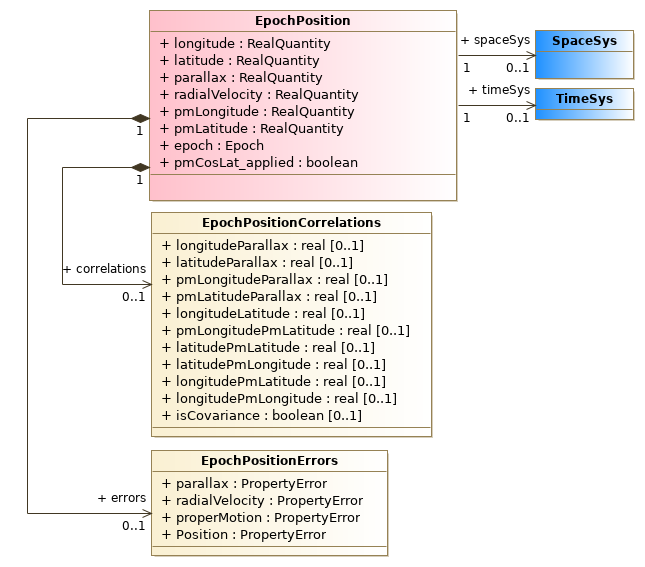
\includegraphics[width=1.0\textwidth]{../model/EpochPosition.png}
        \caption{Class EpochPosition}
        \label{fig:EpochPosition}
      \end{figure}

    
  \label{sect:EpochPosition}
    This class (fig \ref{fig:EpochPosition}) is a view of \texttt{Astronomical Coordinates and Coordinate Systems} \citep{2022ivoa.specQ1004R} components that have been put together to form a consistent description of the position of an object moving over time. It consists of a celestial position, a proper motion, a radial velocity and a parallax. All components share the same coordinate systems for both time and space coordinates. \begin{itemize} \item Both position and proper motion reuse \texttt{coords:LonLatPoint} elements. \item The space coordinate system is imported from \texttt{coords:spaceSys}. \item The time coordinate system is imported from \texttt{coords:timeSys}. \end{itemize} The \texttt{EpochPosition} error is modeled by specific classes supporting covariance and/or correlation between components. All individual components have their own units which must be consistent to each others. This consistency is not enforced by the model. Possible correlations between \texttt{EpochPosition} parameters are handle by the \texttt{EpochPositionCorrelation} class.

    \subsubsection{EpochPosition.longitude}
      \textbf{vodml-id: EpochPosition.longitude} \newline
      \textbf{type: \hyperref[sect:ivoa]{ivoa:RealQuantity}} \newline
      \textbf{multiplicity: 1} \newline
      The longitude of the Point, as a Quantity with angular units (see \texttt{coords:LonLatPoint.lon}.

    \subsubsection{EpochPosition.latitude}
      \textbf{vodml-id: EpochPosition.latitude} \newline
      \textbf{type: \hyperref[sect:ivoa]{ivoa:RealQuantity}} \newline
      \textbf{multiplicity: 1} \newline
      The latitude of the Point, as a Quantity with angular units (see \texttt{coords:LonLatPoint.lat}.

    \subsubsection{EpochPosition.parallax}
      \textbf{vodml-id: EpochPosition.parallax} \newline
      \textbf{type: \hyperref[sect:ivoa]{ivoa:RealQuantity}} \newline
      \textbf{multiplicity: 1} \newline
      The measured parallax in the coordinate system of the \texttt{EpochPosition} instance.

    \subsubsection{EpochPosition.radialVelocity}
      \textbf{vodml-id: EpochPosition.radialVelocity} \newline
      \textbf{type: \hyperref[sect:ivoa]{ivoa:RealQuantity}} \newline
      \textbf{multiplicity: 1} \newline
      The measured Velocity along of the radius axis (see \texttt{meas:Velocity.coord} in \cite{2022ivoa.spec.1004R}).

    \subsubsection{EpochPosition.pmLongitude}
      \textbf{vodml-id: EpochPosition.pmLongitude} \newline
      \textbf{type: \hyperref[sect:ivoa]{ivoa:RealQuantity}} \newline
      \textbf{multiplicity: 1} \newline
      Velocity along the longitude axis in angular distance per unit time (see \texttt{meas:ProperMotion.coord}). The current version of the model only allows a representation in the Polar coordinate space.

    \subsubsection{EpochPosition.pmLatitude}
      \textbf{vodml-id: EpochPosition.pmLatitude} \newline
      \textbf{type: \hyperref[sect:ivoa]{ivoa:RealQuantity}} \newline
      \textbf{multiplicity: 1} \newline
      Velocity along the latitude axis in angular distance per unit time (see \texttt{meas:ProperMotion.coord}). The current version of the model only allows a representation in the Polar coordinate space.

    \subsubsection{EpochPosition.epoch}
      \textbf{vodml-id: EpochPosition.epoch} \newline
      \textbf{type: coords:Epoch} \newline
      \textbf{multiplicity: 1} \newline
      Position epoch expressed within the common time system (see \texttt{coords:epoch})

    \subsubsection{EpochPosition.pmCosLat\_applied}
      \textbf{vodml-id: EpochPosition.pmCosLat\_applied} \newline
      \textbf{type: \hyperref[sect:ivoa]{ivoa:boolean}} \newline
      \textbf{multiplicity: 1} \newline
      It is common, though not universal, practice to quote longitudinal proper motion pre-multiplied by cos(latitude) so that the magnitude of the quantity is not affected by its longitudinal position. We do not constrain the value to one form or the other in this model. Instead, this flag enables providers to convey whether or not the factor has been applied (see \texttt{meas:ProperMotion.cosLat\_applied})

    \subsubsection{EpochPosition.errors}
      \textbf{vodml-id: EpochPosition.errors} \newline
      \textbf{type: \hyperref[sect:EpochPositionErrors]{mango:EpochPositionErrors}} \newline
      \textbf{multiplicity: 0..1} \newline
      Reference to the combined errors of the \texttt{EpochPosition} components.

    \subsubsection{EpochPosition.correlations}
      \textbf{vodml-id: EpochPosition.correlations} \newline
      \textbf{type: \hyperref[sect:EpochPositionCorrelations]{mango:EpochPositionCorrelations}} \newline
      \textbf{multiplicity: 0..1} \newline
      Reference to the correlations between the \texttt{EpochPosition} components.

    \subsubsection{EpochPosition.spaceSys}
      \textbf{vodml-id: EpochPosition.spaceSys} \newline
      \textbf{type: coords:SpaceSys} \newline
      \textbf{multiplicity: 0..1} \newline
      System that applies the space coordinates.

    \subsubsection{EpochPosition.timeSys}
      \textbf{vodml-id: EpochPosition.timeSys} \newline
      \textbf{type: coords:TimeSys} \newline
      \textbf{multiplicity: 0..1} \newline
      System that applies the time coordinates (the epoch).

  \subsection{EpochPositionCorrelations}
  \label{sect:EpochPositionCorrelations}
    Class holder for the correlation coefficients between the \texttt{EpochPosition} components.

    \subsubsection{EpochPositionCorrelations.longitudeParallax}
      \textbf{vodml-id: EpochPositionCorrelations.longitudeParallax} \newline
      \textbf{type: \hyperref[sect:ivoa]{ivoa:real}} \newline
      \textbf{multiplicity: 0..1} \newline
      Correlation (or covariance) coefficient between the position longitude and the parallax

    \subsubsection{EpochPositionCorrelations.latitudeParallax}
      \textbf{vodml-id: EpochPositionCorrelations.latitudeParallax} \newline
      \textbf{type: \hyperref[sect:ivoa]{ivoa:real}} \newline
      \textbf{multiplicity: 0..1} \newline
      Correlation (or covariance) coefficient between the position latitude and the parallax

    \subsubsection{EpochPositionCorrelations.pmLongitudeParallax}
      \textbf{vodml-id: EpochPositionCorrelations.pmLongitudeParallax} \newline
      \textbf{type: \hyperref[sect:ivoa]{ivoa:real}} \newline
      \textbf{multiplicity: 0..1} \newline
      Correlation (or covariance) coefficient between the proper motion longitude and the parallax

    \subsubsection{EpochPositionCorrelations.pmLatitudeParallax}
      \textbf{vodml-id: EpochPositionCorrelations.pmLatitudeParallax} \newline
      \textbf{type: \hyperref[sect:ivoa]{ivoa:real}} \newline
      \textbf{multiplicity: 0..1} \newline
      Correlation (or covariance) coefficient between the proper motion latitude and the parallax

    \subsubsection{EpochPositionCorrelations.longitudeLatitude}
      \textbf{vodml-id: EpochPositionCorrelations.longitudeLatitude} \newline
      \textbf{type: \hyperref[sect:ivoa]{ivoa:real}} \newline
      \textbf{multiplicity: 0..1} \newline
      Correlation (or covariance) coefficient between the position longitude and the position latitude

    \subsubsection{EpochPositionCorrelations.pmLongitudePmLatitude}
      \textbf{vodml-id: EpochPositionCorrelations.pmLongitudePmLatitude} \newline
      \textbf{type: \hyperref[sect:ivoa]{ivoa:real}} \newline
      \textbf{multiplicity: 0..1} \newline
      Correlation (or covariance) coefficient between the proper motion longitude and the proper motion latitude

    \subsubsection{EpochPositionCorrelations.latitudePmLatitude}
      \textbf{vodml-id: EpochPositionCorrelations.latitudePmLatitude} \newline
      \textbf{type: \hyperref[sect:ivoa]{ivoa:real}} \newline
      \textbf{multiplicity: 0..1} \newline
      Correlation (or covariance) coefficient between the position latitude and the proper motion latitude

    \subsubsection{EpochPositionCorrelations.latitudePmLongitude}
      \textbf{vodml-id: EpochPositionCorrelations.latitudePmLongitude} \newline
      \textbf{type: \hyperref[sect:ivoa]{ivoa:real}} \newline
      \textbf{multiplicity: 0..1} \newline
      Correlation (or covariance) coefficient between the position latitude and the proper motion longitude

    \subsubsection{EpochPositionCorrelations.longitudePmLatitude}
      \textbf{vodml-id: EpochPositionCorrelations.longitudePmLatitude} \newline
      \textbf{type: \hyperref[sect:ivoa]{ivoa:real}} \newline
      \textbf{multiplicity: 0..1} \newline
      Correlation (or covariance) coefficient between the position longitude and the proper motion latitude

    \subsubsection{EpochPositionCorrelations.longitudePmLongitude}
      \textbf{vodml-id: EpochPositionCorrelations.longitudePmLongitude} \newline
      \textbf{type: \hyperref[sect:ivoa]{ivoa:real}} \newline
      \textbf{multiplicity: 0..1} \newline
      Correlation (or covariance) coefficient between the position longitude and the proper motion longitude

    \subsubsection{EpochPositionCorrelations.isCovariance}
      \textbf{vodml-id: EpochPositionCorrelations.isCovariance} \newline
      \textbf{type: \hyperref[sect:ivoa]{ivoa:boolean}} \newline
      \textbf{multiplicity: 0..1} \newline
      Boolean telling whether the correlations must be interpreted as covariance or as correlation coefficients.

  \subsection{EpochPositionErrors}
  \label{sect:EpochPositionErrors}
    Class holder for the errors of the EpochPosition attributes

    \subsubsection{EpochPositionErrors.parallax}
      \textbf{vodml-id: EpochPositionErrors.parallax} \newline
      \textbf{type: \hyperref[sect:error.PropertyError]{mango:error.PropertyError}} \newline
      \textbf{multiplicity: 1} \newline
      Parallax error. This error is meant to be symmetrical in the current model version.

    \subsubsection{EpochPositionErrors.radialVelocity}
      \textbf{vodml-id: EpochPositionErrors.radialVelocity} \newline
      \textbf{type: \hyperref[sect:error.PropertyError]{mango:error.PropertyError}} \newline
      \textbf{multiplicity: 1} \newline
      Error in the radial velocity. This error is meant to be symmetrical in the current model version.

    \subsubsection{EpochPositionErrors.properMotion}
      \textbf{vodml-id: EpochPositionErrors.properMotion} \newline
      \textbf{type: \hyperref[sect:error.PropertyError]{mango:error.PropertyError}} \newline
      \textbf{multiplicity: 1} \newline
      Position error; can be an ellipse, a correlation matrix or a covariance matrix.

    \subsubsection{EpochPositionErrors.Position}
      \textbf{vodml-id: EpochPositionErrors.Position} \newline
      \textbf{type: \hyperref[sect:error.PropertyError]{mango:error.PropertyError}} \newline
      \textbf{multiplicity: 1} \newline
      Position error; can be an ellipse, a correlation matrix or a covariance matrix.

  \subsection{Label}
  \label{sect:Label}
    Free text label seen as a MANGO object property.

    \subsubsection{Label.text}
      \textbf{vodml-id: Label.text} \newline
      \textbf{type: \hyperref[sect:ivoa]{ivoa:string}} \newline
      \textbf{multiplicity: 1} \newline
      Text of label property of the MANGO object.

  \subsection{MangoObject}
  \label{sect:MangoObject}
    Central model class: applied to a data table, each row can be modelled as a \texttt{MangoObject} instance. Each \texttt{MangoObject} hosts a collection of physical or calculated parameters, a description of the data origin and an identifier.

    \subsubsection{MangoObject.identifier}
      \textbf{vodml-id: MangoObject.identifier} \newline
      \textbf{type: \hyperref[sect:ivoa]{ivoa:string}} \newline
      \textbf{multiplicity: 1} \newline
      Unique identifier of the \texttt{MangoObject}. The uniqueness of that identifier is not managed by the model. The format is free.

    \subsubsection{MangoObject.propertyDock}
      \textbf{vodml-id: MangoObject.propertyDock} \newline
      \textbf{type: \hyperref[sect:Property]{mango:Property}} \newline
      \textbf{multiplicity: 0..*} \newline
      Reference to the open-ended collection of the \texttt{MangoObject} properties (physical or calculated).

    \subsubsection{MangoObject.dataOrigin}
      \textbf{vodml-id: MangoObject.dataOrigin} \newline
      \textbf{type: \hyperref[sect:dataorigin.DataOrigin]{mango:dataorigin.DataOrigin}} \newline
      \textbf{multiplicity: 0..1} \newline
      Reference to the description of the origin of the \texttt{MangoObject}.

    \subsubsection{MangoObject.associatedMangoObjects}
      \textbf{vodml-id: MangoObject.associatedMangoObjects} \newline
      \textbf{type: \hyperref[sect:AssociatedMangoObject]{mango:AssociatedMangoObject}} \newline
      \textbf{multiplicity: 0..*} \newline
      Abstract reference to a particular dataset associated to the MANGO entity. This class is used to specify the type of the associated dataset as well as its role.

  \subsection{PhotometricProperty}
  \label{sect:PhotometricProperty}
    Super class for all photometric properties of the \texttt{MangoObject}.

    \subsubsection{PhotometricProperty.value}
      \textbf{vodml-id: PhotometricProperty.value} \newline
      \textbf{type: \hyperref[sect:ivoa]{ivoa:RealQuantity}} \newline
      \textbf{multiplicity: 1} \newline
      Value of the photometric property associated with a photometric calibration as defined by the \texttt{PhotDM} model.

    \subsubsection{PhotometricProperty.error}
      \textbf{vodml-id: PhotometricProperty.error} \newline
      \textbf{type: meas:Uncertainty} \newline
      \textbf{multiplicity: 1} \newline
      Error on the \texttt{PhotometricProperty}, imported from \texttt{meas:Uncertainty}.

  \subsection{PhysicalProperty}
  \label{sect:PhysicalProperty}
    Place holder for any quantity that can be hold by measure classes as defined in the \texttt{Astronomical Measurements Model}.

    \subsubsection{PhysicalProperty.calibrationLevel}
      \textbf{vodml-id: PhysicalProperty.calibrationLevel} \newline
      \textbf{type: \hyperref[sect:CalibrationLevel]{mango:CalibrationLevel}} \newline
      \textbf{multiplicity: 1} \newline
      Calibration level of the property as defined in ObsCore \citep{2011ivoa.spec.1028T}.

    \subsubsection{PhysicalProperty.measure}
      \textbf{vodml-id: PhysicalProperty.measure} \newline
      \textbf{type: meas:Measure} \newline
      \textbf{multiplicity: 1} \newline
      Instance of \texttt{Astronomical Measurements Model} that holds the Property value(s).

  \subsection{Property}
  \label{sect:Property}
    Class holder for a particular property, either physical or calculated, of the MANGO object. This class specifies both type and role of the property, and hosts the property instance itself.

    \noindent \textbf{constraint} \newline
    \indent    \textbf{detail: Property.One association at the time
 }\newline


    \subsubsection{Property.semantics}
      \textbf{vodml-id: Property.semantics} \newline
      \textbf{type: \hyperref[sect:VocabularyTerm]{mango:VocabularyTerm}} \newline
      \textbf{multiplicity: 1} \newline
      Reference to a semantic concept giving the nature of the property or of the set made of the property and its associated properties. The semantics field contains a URI for a concept that describes the meaning of the property. This attribute is intended to be machine-readable and to assist automated link selection, presentation, and usage. The value is always interpreted as a URI; relative URIs (Berners-Lee and Fielding et al., 2005) are completed using the base URI of the core DataLink vocabulary, http://www.ivoa.net/rdf/datalink/core. Terms from this vocabulary must always be written as relative URIs. This means that for concepts from the core vocabulary, the value in the semantics fieldz always starts with a hash. (datalink1.1). The semantic concept apply to a single property or to the set made of the property and its associated properties (e.g. position and flag).

    \subsubsection{Property.description}
      \textbf{vodml-id: Property.description} \newline
      \textbf{type: \hyperref[sect:ivoa]{ivoa:string}} \newline
      \textbf{multiplicity: 1} \newline
      Free text description of the property or of the set made of the property and its associated properties.

    \subsubsection{Property.associatedProperties}
      \textbf{vodml-id: Property.associatedProperties} \newline
      \textbf{type: \hyperref[sect:Property]{mango:Property}} \newline
      \textbf{multiplicity: 1..*} \newline
      Open-ended collection of MANGO properties associated with the \texttt{MangoObject}. These relationships are typically used to associate physical properties with time stamps and/or quality factors.

  \subsection{Shape}
  \label{sect:Shape}
    Description of the spatial extension of the MANGO object (for e.g. dust clouds)

    \subsubsection{Shape.shape}
      \textbf{vodml-id: Shape.shape} \newline
      \textbf{type: \hyperref[sect:ivoa]{ivoa:string}} \newline
      \textbf{multiplicity: 1} \newline
      String serialization of the spatial extension of the \texttt{MangoObject}

    \subsubsection{Shape.serialization}
      \textbf{vodml-id: Shape.serialization} \newline
      \textbf{type: \hyperref[sect:ShapeSerialization]{mango:ShapeSerialization}} \newline
      \textbf{multiplicity: 1} \newline
      Serialization mode of the spatial extension of the MANGO entity

    \subsubsection{Shape.spaceSys}
      \textbf{vodml-id: Shape.spaceSys} \newline
      \textbf{type: coords:SpaceSys} \newline
      \textbf{multiplicity: 0..1} \newline
      Coordinate system that applies for the shape

  \subsection{Status}
  \label{sect:Status}
    Property representing a status defined by a integer number that can only take on a defined number of values, each with its own description. Boolean status can be represented by \texttt{StatusValues} with 2 values e.g. 0 for False and 1 for True.

    \subsubsection{Status.status}
      \textbf{vodml-id: Status.status} \newline
      \textbf{type: \hyperref[sect:ivoa]{ivoa:integer}} \newline
      \textbf{multiplicity: 1} \newline
      Actual value of the status

    \subsubsection{Status.allowedValues}
      \textbf{vodml-id: Status.allowedValues} \newline
      \textbf{type: \hyperref[sect:StatusValues]{mango:StatusValues}} \newline
      \textbf{multiplicity: 0..1} \newline
      List of the allowed values for the status. Each value has its own free text description.

  \subsection{StatusValue}
  \label{sect:StatusValue}
    Value allowed for a status; contain the value with a free text description.

    \subsubsection{StatusValue.value}
      \textbf{vodml-id: StatusValue.value} \newline
      \textbf{type: \hyperref[sect:ivoa]{ivoa:integer}} \newline
      \textbf{multiplicity: 1} \newline
      Allowed value for a \texttt{Status}

    \subsubsection{StatusValue.description}
      \textbf{vodml-id: StatusValue.description} \newline
      \textbf{type: \hyperref[sect:ivoa]{ivoa:string}} \newline
      \textbf{multiplicity: 1} \newline
      Free text description of the allowed value for a \texttt{Status}

  \subsection{StatusValues}
  \label{sect:StatusValues}
    Class holder for the list of the allowed values for the status.

    \subsubsection{StatusValues.values}
      \textbf{vodml-id: StatusValues.values} \newline
      \textbf{type: \hyperref[sect:StatusValue]{mango:StatusValue}} \newline
      \textbf{multiplicity: 1..*} \newline
      List of the allowed values for the status; each value has its own textual description.

  \subsection{VocabularyTerm}
  \label{sect:VocabularyTerm}
    Class holder for a term of a standardized vocabulary that applies to a property.

    \subsubsection{VocabularyTerm.uri}
      \textbf{vodml-id: VocabularyTerm.uri} \newline
      \textbf{type: \hyperref[sect:ivoa]{ivoa:string}} \newline
      \textbf{multiplicity: 1} \newline
      URI the vocabulary term

    \subsubsection{VocabularyTerm.label}
      \textbf{vodml-id: VocabularyTerm.label} \newline
      \textbf{type: \hyperref[sect:ivoa]{ivoa:string}} \newline
      \textbf{multiplicity: 1} \newline
      Label attached to the vocabulary term. This is necessary because the URI may not contain any explicit label. This was the case for the IUA vocabulary until the Registry WG introduced rewriting rules that fix the issue.

  \subsection{ShapeFrame}
  \label{sect:ShapeFrame}

  Possible schemes to encode a shape in a string

  \noindent \underline{Enumeration Literals}
  \vspace{-\parsep}
  \small
  \begin{itemize}
  
    \item[\textbf{STC\_S}]: \textbf{vodml-id:} ShapeFrame.STC\_S \newline
          \textbf{description:} MOC serialization
    \item[\textbf{MOC}]: \textbf{vodml-id:} ShapeFrame.MOC \newline
          \textbf{description:} MOC serialization
  \end{itemize}
  \normalsize


  \subsection{ShapeSerialization}
  \label{sect:ShapeSerialization}

  Enumeration of the supported serialization modes for the shapes

  \noindent \underline{Enumeration Literals}
  \vspace{-\parsep}
  \small
  \begin{itemize}
  
    \item[\textbf{MOC}]: \textbf{vodml-id:} ShapeSerialization.MOC \newline
          \textbf{description:} Label indicating that the shape has been serialized as a S-MOC
    \item[\textbf{STCS}]: \textbf{vodml-id:} ShapeSerialization.STCS \newline
          \textbf{description:} Label indicating that the shape has been serialized as a STC-S \citep{2007ivoa.spec.1030R} string
    \item[\textbf{POLYGON}]: \textbf{vodml-id:} ShapeSerialization.POLYGON \newline
          \textbf{description:} Label indicating that the shape has been serialized as a polygon (cf xtypes)
  \end{itemize}
  \normalsize


  \subsection{CalibrationLevel}
  \label{sect:CalibrationLevel}

  Enumeration of different possible calibration status of the property as defined in Obscore

  \noindent \underline{Enumeration Literals}
  \vspace{-\parsep}
  \small
  \begin{itemize}
  
    \item[\textbf{Raw}]: \textbf{vodml-id:} CalibrationLevel.Raw \newline
          \textbf{description:} Raw instrumental data, in a proprietary or internal data provider defined format, that needs instrument specific tools to be handled (ObsCore)
    \item[\textbf{Instrumental}]: \textbf{vodml-id:} CalibrationLevel.Instrumental \newline
          \textbf{description:} Instrumental data in a standard format which could be manipulated with standard astronomical packages (ObsCore).
    \item[\textbf{Calibrated}]: \textbf{vodml-id:} CalibrationLevel.Calibrated \newline
          \textbf{description:} Science ready data with the instrument signature removed (ObsCore)
  \end{itemize}
  \normalsize


  \subsection{ColorDefinition}
  \label{sect:ColorDefinition}

  Enumeration of the different types of colors supported by the model.

  \noindent \underline{Enumeration Literals}
  \vspace{-\parsep}
  \small
  \begin{itemize}
  
    \item[\textbf{ColorIndex}]: \textbf{vodml-id:} ColorDefinition.ColorIndex \newline
          \textbf{description:} Difference of magnitudes: typically $M_B - M_v$
    \item[\textbf{HardnessRatio}]: \textbf{vodml-id:} ColorDefinition.HardnessRatio \newline
          \textbf{description:} Normalized ratio of fluxes: $(F_{EB2} - F_{EB1}) / (F_{EB2} + F_{EB1})$
  \end{itemize}
  \normalsize


\pagebreak
\section{Package: error }
  \begin{figure}[h]
    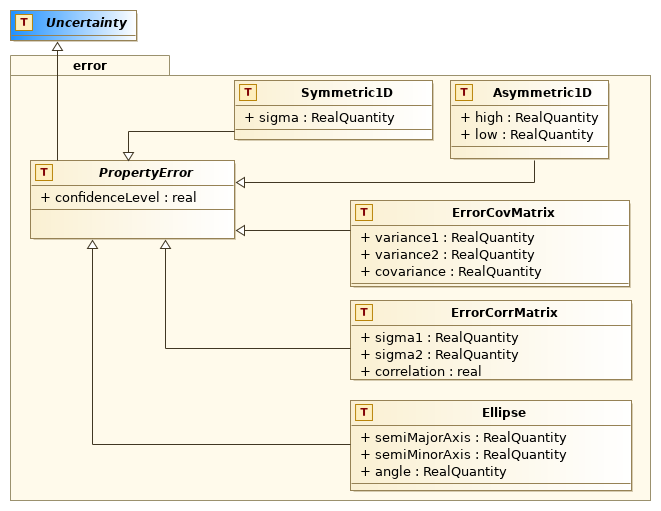
\includegraphics[width=1.0\textwidth]{../model/error.png}
    \caption{package error}
    \label{fig:error}
  \end{figure}



  % INSERT FIGURE HERE
  %\begin{figure}[h]
  %\begin{center}
  %  \includegraphics[width=\textwidth]{????.png}
  %  \caption{???}\label{fig:????}
  %\end{center}
  %\end{figure}

  The \texttt{error} package (fig \ref{fig:error}) groups the MANGO built-in error classes. All these classes are derived from \texttt{meas:Uncertainty} to make them reusable by \texttt{meas:Measure} instances. Mango errors all have an attribute that specifies the confidence level

  \subsection{Asymmetric1D}
  \label{sect:error.Asymmetric1D}
    Asymmetric error for 1D parameters

    \subsubsection{Asymmetric1D.high}
      \textbf{vodml-id: error.Asymmetric1D.high} \newline
      \textbf{type: \hyperref[sect:ivoa]{ivoa:RealQuantity}} \newline
      \textbf{multiplicity: 1} \newline
      High limit for the asymmetric error for 1D parameters

    \subsubsection{Asymmetric1D.low}
      \textbf{vodml-id: error.Asymmetric1D.low} \newline
      \textbf{type: \hyperref[sect:ivoa]{ivoa:RealQuantity}} \newline
      \textbf{multiplicity: 1} \newline
      Low limit for the asymmetric error for 1D parameters

  \subsection{Ellipse}
  \label{sect:error.Ellipse}
    Elliptic error for 2D parameters such as sky positions. Major axis and minor axis have their own units, which must be the same for both. This is not enforced by the model. The definition of the ellipse attribute is imported from \texttt{coords:Ellipse}.

    \subsubsection{Ellipse.semiMajorAxis}
      \textbf{vodml-id: error.Ellipse.semiMajorAxis} \newline
      \textbf{type: \hyperref[sect:ivoa]{ivoa:RealQuantity}} \newline
      \textbf{multiplicity: 1} \newline
      Half of the ellipse major axis

    \subsubsection{Ellipse.semiMinorAxis}
      \textbf{vodml-id: error.Ellipse.semiMinorAxis} \newline
      \textbf{type: \hyperref[sect:ivoa]{ivoa:RealQuantity}} \newline
      \textbf{multiplicity: 1} \newline
      Half of the ellipse minor axis

    \subsubsection{Ellipse.angle}
      \textbf{vodml-id: error.Ellipse.angle} \newline
      \textbf{type: \hyperref[sect:ivoa]{ivoa:RealQuantity}} \newline
      \textbf{multiplicity: 1} \newline
      Angle between the North Polar Cape (NCP) and the major axis. This angle must be positive taking into account that angles are positive from North to the East. The angle has its own unit.

  \subsection{ErrorCorrMatrix}
  \label{sect:error.ErrorCorrMatrix}
    Correlation matrix for the error of a 2D quantities. The correlation matrix is symmetrical.

    \subsubsection{ErrorCorrMatrix.sigma1}
      \textbf{vodml-id: error.ErrorCorrMatrix.sigma1} \newline
      \textbf{type: \hyperref[sect:ivoa]{ivoa:RealQuantity}} \newline
      \textbf{multiplicity: 1} \newline
      Error on the first dimension (right ascension in case of sky coordinates)

    \subsubsection{ErrorCorrMatrix.sigma2}
      \textbf{vodml-id: error.ErrorCorrMatrix.sigma2} \newline
      \textbf{type: \hyperref[sect:ivoa]{ivoa:RealQuantity}} \newline
      \textbf{multiplicity: 1} \newline
      Error on the second dimension (declination in case of sky coordinates)

    \subsubsection{ErrorCorrMatrix.correlation}
      \textbf{vodml-id: error.ErrorCorrMatrix.correlation} \newline
      \textbf{type: \hyperref[sect:ivoa]{ivoa:real}} \newline
      \textbf{multiplicity: 1} \newline
      Correlation coefficient between the 2 axis

  \subsection{ErrorCovMatrix}
  \label{sect:error.ErrorCovMatrix}
    Covariance matrix for the error of a 2D quantities. The covariance matrix is symmetrical.

    \subsubsection{ErrorCovMatrix.variance1}
      \textbf{vodml-id: error.ErrorCovMatrix.variance1} \newline
      \textbf{type: \hyperref[sect:ivoa]{ivoa:RealQuantity}} \newline
      \textbf{multiplicity: 1} \newline
      Variance of the first dimension (right ascension in case of sky coordinates)

    \subsubsection{ErrorCovMatrix.variance2}
      \textbf{vodml-id: error.ErrorCovMatrix.variance2} \newline
      \textbf{type: \hyperref[sect:ivoa]{ivoa:RealQuantity}} \newline
      \textbf{multiplicity: 1} \newline
      Variance of the second dimension (declination in case of sky coordinates)

    \subsubsection{ErrorCovMatrix.covariance}
      \textbf{vodml-id: error.ErrorCovMatrix.covariance} \newline
      \textbf{type: \hyperref[sect:ivoa]{ivoa:RealQuantity}} \newline
      \textbf{multiplicity: 1} \newline
      Covariance of the 2 axis

  \subsection{PropertyError (Abstract)}
  \label{sect:error.PropertyError}
    Root (abstract) class of the errors that can be attached to a MANGO property. The class inherits from \texttt{meas:uncertainty} in order to be usable in the context of properties based on \texttt{Measures} classes.

    \subsubsection{PropertyError.confidenceLevel}
      \textbf{vodml-id: error.PropertyError.confidenceLevel} \newline
      \textbf{type: \hyperref[sect:ivoa]{ivoa:real}} \newline
      \textbf{multiplicity: 1} \newline
      Confidence level of the error. The confidence level must be in $[0, 1]$ (not enforced by the VO-DML schema).

    \subsubsection{PropertyError.distribution}
      \textbf{vodml-id: error.PropertyError.distribution} \newline
      \textbf{type: \hyperref[sect:ivoa]{ivoa:string}} \newline
      \textbf{multiplicity: 1} \newline
      TODO : Missing description : please, update your UML model asap.

  \subsection{Symmetric1D}
  \label{sect:error.Symmetric1D}
    Symmetric error for 1D parameters

    \subsubsection{Symmetric1D.sigma}
      \textbf{vodml-id: error.Symmetric1D.sigma} \newline
      \textbf{type: \hyperref[sect:ivoa]{ivoa:RealQuantity}} \newline
      \textbf{multiplicity: 1} \newline
      Amplitude of the symmetric error on a one-dimensional parameter

\pagebreak
\section{Package: dataorigin }
  \begin{figure}[h]
    \includegraphics[width=1.0\textwidth]{../model/dataorigin.png}
    \caption{package dataorigin}
    \label{fig:dataorigin}
  \end{figure}



  % INSERT FIGURE HERE
  %\begin{figure}[h]
  %\begin{center}
  %  \includegraphics[width=\textwidth]{????.png}
  %  \caption{???}\label{fig:????}
  %\end{center}
  %\end{figure}

  Package grouping together all the components needed to model the origin of \texttt{MangoObject} (fig \ref{fig:dataorigin}).

  \subsection{Article}
  \label{sect:dataorigin.Article}
    Reference article for the MANGO entity

    \subsubsection{Article.editor}
      \textbf{vodml-id: dataorigin.Article.editor} \newline
      \textbf{type: \hyperref[sect:ivoa]{ivoa:string}} \newline
      \textbf{multiplicity: 1} \newline
      Name of the article editor

    \subsubsection{Article.code}
      \textbf{vodml-id: dataorigin.Article.code} \newline
      \textbf{type: \hyperref[sect:ivoa]{ivoa:string}} \newline
      \textbf{multiplicity: 1} \newline
      Bibcode or DOI of the reference article

  \subsection{DataOrigin}
  \label{sect:dataorigin.DataOrigin}
    Class representing the origin of the data following the DCP note

    \subsubsection{DataOrigin.citation}
      \textbf{vodml-id: dataorigin.DataOrigin.citation} \newline
      \textbf{type: \hyperref[sect:ivoa]{ivoa:string}} \newline
      \textbf{multiplicity: 1} \newline
      Dataset identifier that can be used for citation (e.g. DOI)

    \subsubsection{DataOrigin.reference\_url}
      \textbf{vodml-id: dataorigin.DataOrigin.reference\_url} \newline
      \textbf{type: \hyperref[sect:ivoa]{ivoa:string}} \newline
      \textbf{multiplicity: 1} \newline
      Dataset landing page

    \subsubsection{DataOrigin.resource\_version}
      \textbf{vodml-id: dataorigin.DataOrigin.resource\_version} \newline
      \textbf{type: \hyperref[sect:ivoa]{ivoa:string}} \newline
      \textbf{multiplicity: 1} \newline
      Dataset version

    \subsubsection{DataOrigin.creator}
      \textbf{vodml-id: dataorigin.DataOrigin.creator} \newline
      \textbf{type: \hyperref[sect:ivoa]{ivoa:string}} \newline
      \textbf{multiplicity: 1} \newline
      Person(s) mainly involved in the creation of the resource, generally the author

    \subsubsection{DataOrigin.cites}
      \textbf{vodml-id: dataorigin.DataOrigin.cites} \newline
      \textbf{type: \hyperref[sect:ivoa]{ivoa:string}} \newline
      \textbf{multiplicity: 1} \newline
      Identifier (IVOID, DOI or Bibcode) of a second Resource using relation of type \texttt{cites} (\url{https://www.ivoa.net/rdf/voresource/relationship\_type/})

    \subsubsection{DataOrigin.is\_derived\_from}
      \textbf{vodml-id: dataorigin.DataOrigin.is\_derived\_from} \newline
      \textbf{type: \hyperref[sect:ivoa]{ivoa:string}} \newline
      \textbf{multiplicity: 1} \newline
      Identifier (IVOID, DOI or Bibcode) of a second resource using relation of type \texttt{is\_derived\_from} (\url{https://www.ivoa.net/rdf/voresource/relationship\_type/})

    \subsubsection{DataOrigin.original\_date}
      \textbf{vodml-id: dataorigin.DataOrigin.original\_date} \newline
      \textbf{type: \hyperref[sect:ivoa]{ivoa:datetime}} \newline
      \textbf{multiplicity: 1} \newline
      Date of the original resource from which the MANGO object is derived

    \subsubsection{DataOrigin.query}
      \textbf{vodml-id: dataorigin.DataOrigin.query} \newline
      \textbf{type: \hyperref[sect:dataorigin.QueryOrigin]{mango:dataorigin.QueryOrigin}} \newline
      \textbf{multiplicity: 0..1} \newline
      Description of the request from which the data originates.

    \subsubsection{DataOrigin.rights}
      \textbf{vodml-id: dataorigin.DataOrigin.rights} \newline
      \textbf{type: \hyperref[sect:dataorigin.License]{mango:dataorigin.License}} \newline
      \textbf{multiplicity: 0..1} \newline
      Reference to the rights that apply to the data.

    \subsubsection{DataOrigin.article}
      \textbf{vodml-id: dataorigin.DataOrigin.article} \newline
      \textbf{type: \hyperref[sect:dataorigin.Article]{mango:dataorigin.Article}} \newline
      \textbf{multiplicity: 0..1} \newline
      Reference to the article from which the data originates.

  \subsection{License}
  \label{sect:dataorigin.License}
    Place holder for the license covering the MANGO instance

    \subsubsection{License.rights\_uri}
      \textbf{vodml-id: dataorigin.License.rights\_uri} \newline
      \textbf{type: \hyperref[sect:ivoa]{ivoa:string}} \newline
      \textbf{multiplicity: 1} \newline
      Licence URI. Following Registry practice, this should come from SPDX https://spdx.org/licenses/, though Creative Commons URLs https://creativecommons.org are also admitted.

    \subsubsection{License.rights}
      \textbf{vodml-id: dataorigin.License.rights} \newline
      \textbf{type: \hyperref[sect:ivoa]{ivoa:string}} \newline
      \textbf{multiplicity: 1} \newline
      License or Copyright text

  \subsection{QueryOrigin}
  \label{sect:dataorigin.QueryOrigin}
    Description of the query the MANGO instance results from.

    \subsubsection{QueryOrigin.ivoid}
      \textbf{vodml-id: dataorigin.QueryOrigin.ivoid} \newline
      \textbf{type: \hyperref[sect:ivoa]{ivoa:string}} \newline
      \textbf{multiplicity: 1} \newline
      IVOID of the underlying data collection

    \subsubsection{QueryOrigin.publisher}
      \textbf{vodml-id: dataorigin.QueryOrigin.publisher} \newline
      \textbf{type: \hyperref[sect:ivoa]{ivoa:string}} \newline
      \textbf{multiplicity: 1} \newline
      Data center that produced the MANGO instance

    \subsubsection{QueryOrigin.server\_software}
      \textbf{vodml-id: dataorigin.QueryOrigin.server\_software} \newline
      \textbf{type: \hyperref[sect:ivoa]{ivoa:string}} \newline
      \textbf{multiplicity: 1} \newline
      Version of the software the produced the MANGO object instance. It is encouraged to follow \url{https://ivoa.net/documents/Notes/softid/index.html}.

    \subsubsection{QueryOrigin.service\_protocol}
      \textbf{vodml-id: dataorigin.QueryOrigin.service\_protocol} \newline
      \textbf{type: \hyperref[sect:ivoa]{ivoa:string}} \newline
      \textbf{multiplicity: 1} \newline
      IVOID \citep{2007ivoa.spec.0314P} of the protocol through which the data was retrieved

    \subsubsection{QueryOrigin.request}
      \textbf{vodml-id: dataorigin.QueryOrigin.request} \newline
      \textbf{type: \hyperref[sect:ivoa]{ivoa:string}} \newline
      \textbf{multiplicity: 1} \newline
      Full request URL including a query string. For the simple protocols,put the url-encoded form of the query parameters. For TAP queries, use the /sync UWS \citep{2016ivoa.spec.1024H} URL. The format is free for others request types.

    \subsubsection{QueryOrigin.query}
      \textbf{vodml-id: dataorigin.QueryOrigin.query} \newline
      \textbf{type: \hyperref[sect:ivoa]{ivoa:string}} \newline
      \textbf{multiplicity: 1} \newline
      Input query in a formal langage such as ADQL.equest types \citep{2023ivoa.spec.1215M}

    \subsubsection{QueryOrigin.request\_date}
      \textbf{vodml-id: dataorigin.QueryOrigin.request\_date} \newline
      \textbf{type: \hyperref[sect:ivoa]{ivoa:datetime}} \newline
      \textbf{multiplicity: 1} \newline
      Query execution date

    \subsubsection{QueryOrigin.contact}
      \textbf{vodml-id: dataorigin.QueryOrigin.contact} \newline
      \textbf{type: \hyperref[sect:ivoa]{ivoa:string}} \newline
      \textbf{multiplicity: 1} \newline
      Email or URL to contact the publisher